\documentclass{article}

\usepackage[a0paper,portrait,margin=12mm]{geometry}
\usepackage[T1]{fontenc}
\usepackage[utf8]{inputenc}
\usepackage{microtype}
\usepackage{inconsolata}
\usepackage{newtxtext}
\usepackage{amsmath}
\usepackage{amssymb}
\usepackage{booktabs}
\usepackage{graphicx}
\usepackage{xcolor}
\usepackage{tikz}
\usepackage[most]{tcolorbox}
\usepackage{listings}
\usetikzlibrary{arrows.meta,positioning,fit,calc,shapes.geometric}

\pagestyle{empty}

\definecolor{axonblue}{HTML}{12355B}
\definecolor{axoncyan}{HTML}{1C6E8C}
\definecolor{axonorange}{HTML}{D97D0D}
\definecolor{axongreen}{HTML}{4A7C59}
\definecolor{axonpaper}{HTML}{F7F3EA}
\definecolor{axonink}{HTML}{202124}
\definecolor{axonmuted}{HTML}{5E6670}
\definecolor{axoncode}{HTML}{F2EFE7}
\definecolor{axonred}{HTML}{B8331A}

\newcommand{\axon}{\textsc{Axon}}
\newcommand{\graphir}{\textsc{Graph IR}}
\newcommand{\code}[1]{\texttt{#1}}
\newcommand{\postertext}[1]{{\raggedright\fontsize{23}{29}\selectfont #1\par}}

\newcommand{\axonlogo}{%

\begin{tikzpicture}[baseline=-0.55ex,scale=1.22,transform shape]
  \path[fill=white, draw=axonblue, line width=2.9pt, rounded corners=9pt]
    (-1.18,-0.82) -- (-0.56,1.00) -- (0.56,1.00) -- (1.18,-0.82) -- cycle;
  \path[fill=axonblue!5, draw=none, rounded corners=8pt]
    (-0.98,-0.66) -- (-0.46,0.78) -- (0.46,0.78) -- (0.98,-0.66) -- cycle;

  % Lambda as graph: the left stem is control flow, the right stem is data flow.
  \draw[line width=5.2pt, axonblue, line cap=round]
    (-0.55,-0.58) -- (-0.09,0.70);
  \draw[line width=5.2pt, axoncyan, line cap=round]
    (-0.10,0.68) -- (0.63,-0.58);
  \draw[line width=3.2pt, axonorange, line cap=round]
    (-0.34,-0.12) -- (0.40,-0.12);

  \fill[axonblue]   (-0.55,-0.58) circle (0.105cm);
  \fill[axonorange] (-0.09,0.70) circle (0.105cm);
  \fill[axoncyan]   (0.63,-0.58) circle (0.105cm);
  \fill[axongreen]  (-0.34,-0.12) circle (0.085cm);
  \fill[axonred]    (0.40,-0.12) circle (0.085cm);

  \node[font=\bfseries\fontsize{15}{15}\selectfont, text=axonblue] at (0,-1.08) {Axon};
\end{tikzpicture}%
}

\lstdefinelanguage{Axon}{
  morekeywords={do,return,import,true,false,null,scope,for,carry,yield},
  sensitive=true,
  morecomment=[l]{--}
}
\lstset{
  language=Axon,
  basicstyle=\ttfamily\fontsize{19}{21}\selectfont,
  keywordstyle=\color{axonblue}\bfseries,
  commentstyle=\color{axonmuted},
  stringstyle=\color{axongreen},
  columns=fullflexible,
  keepspaces=true,
  showstringspaces=false,
  breaklines=true,
  breakatwhitespace=false,
  frame=none,
  xleftmargin=0.04in,
  xrightmargin=0.04in,
}

\tcbset{
  posterbox/.style={
    enhanced,
    sharp corners=south,
    rounded corners=north,
    colback=white,
    colframe=axonblue,
    boxrule=2.3pt,
    left=5mm,
    right=5mm,
    top=4mm,
    bottom=4mm,
    fonttitle=\bfseries\fontsize{30}{34}\selectfont,
    coltitle=white,
    colbacktitle=axonblue,
    attach boxed title to top left={xshift=4mm,yshift=-1.4mm},
    boxed title style={sharp corners=south,rounded corners=north,boxrule=0pt,colback=axonblue},
  },
  accentbox/.style={
    enhanced,
    colback=axonblue!6,
    colframe=axoncyan,
    boxrule=2pt,
    arc=4mm,
    left=5mm,
    right=5mm,
    top=4mm,
    bottom=4mm,
  },
  codebox/.style={
    enhanced,
    colback=axoncode,
    colframe=axonorange,
    boxrule=1.8pt,
    arc=3mm,
    left=3mm,
    right=3mm,
    top=2mm,
    bottom=2mm,
  }
}

\begin{document}
\pagecolor{axonpaper}
\color{axonink}

\begin{tcolorbox}[enhanced, colback=white, colframe=axonblue, boxrule=3pt, arc=6mm,
  left=8mm,right=8mm,top=7mm,bottom=7mm]
\begin{minipage}[c]{0.15\linewidth}
\centering
{\axonlogo}
\end{minipage}
\begin{minipage}[c]{0.66\linewidth}
\centering
{\fontsize{59}{64}\selectfont\bfseries \axon: Typed Model Programs}\\[1mm]
{\fontsize{38}{43}\selectfont From readable tensor source to structured Graph IR}\\[2mm]
{\fontsize{24}{28}\selectfont source Axon $\rightarrow$ closed flat typed AST $\rightarrow$ typed \graphir{} $\rightarrow$ codegen2/runtime2/pipeline2/tinygrad}
\end{minipage}
\begin{minipage}[c]{0.16\linewidth}
\centering

\includegraphics[width=0.86\linewidth]{sdu_logo.png}\\[2mm]
{\fontsize{18}{21}\selectfont Brainsurgery contributors}
\end{minipage}
\end{tcolorbox}

\vspace{8mm}

\noindent
\begin{minipage}[t]{0.49\linewidth}
\begin{tcolorbox}[posterbox,title={Why Axon?}]
\postertext{\axon{} keeps model-family source compact while preserving the
backend-critical facts: symbolic dimensions, parameter paths, optional caches,
configuration values, typed defaults, and reusable builtin definitions.}
\vspace{3mm}
{\fontsize{21}{27}\selectfont
\begin{tabular}{@{}p{0.27\linewidth}p{0.65\linewidth}@{}}
\toprule
Goal & Mechanism \\
\midrule
Readable source & signatures, \code{do} blocks, pipes, path sugar \\
Typed tensors & \code{Tensor[B,S,D]}, \code{?Cache[B,H,T,DH]} \\
No string IR & semantic AST stages, then typed structured \graphir \\
Portability & one graph contract for torch, runtime, pipeline, tinygrad \\
No model quirks & model-specific handling stays outside compiler core \\
\bottomrule
\end{tabular}
}
\end{tcolorbox}

\vspace{7mm}

\begin{tcolorbox}[posterbox,title={Surface Sugar $\rightarrow$ Flat Core}]
\begin{minipage}[t]{0.49\linewidth}
{\fontsize{22}{26}\selectfont\bfseries Sugared source}
\begin{tcolorbox}[codebox]
\begin{lstlisting}[basicstyle=\ttfamily\fontsize{18}{20}\selectfont]
project :: Tensor[B,S,D] -> Tensor[B,S,O]
project x = do
  y <- Tensor.reshape x shape=[B,S,D]
       |> NN.linear@proj dim=O
  return y
\end{lstlisting}
\end{tcolorbox}
\end{minipage}
\hfill
\begin{minipage}[t]{0.49\linewidth}
{\fontsize{22}{26}\selectfont\bfseries Desugared/flat core}
\begin{tcolorbox}[codebox]
\begin{lstlisting}[basicstyle=\ttfamily\fontsize{18}{20}\selectfont]
project :: Tensor[B,S,D] -> Tensor[B,S,O]
project x = do
  _v1 <- Tensor.reshape x shape=[B,S,D]
  y <- NN.linear @@proj _v1
       dim=O bias=true transpose=false
  return y
\end{lstlisting}
\end{tcolorbox}
\end{minipage}
\vspace{2mm}
{\raggedright\fontsize{22}{28}\selectfont Normalize removes pipes/path sugar; elaborate accounts for defaults; flatten exposes eager evaluation order and absolute or templated paths.\par}
\end{tcolorbox}
\end{minipage}
\hfill
\begin{minipage}[t]{0.49\linewidth}
\begin{tcolorbox}[posterbox,title={Typed Core}]
\postertext{Typecheck2 annotates every expression with type, arity, and
tensor-dimension metadata. Typed flat Axon is the last AST-level representation
before lowering.}
\begin{tcolorbox}[codebox]
\begin{lstlisting}[basicstyle=\ttfamily\fontsize{18}{20}\selectfont]
_v1 <- (Tensor.reshape (x :: Tensor[B,S,D])
          shape=([B,S,D] :: List[Dim])
        :: Tensor[B,S,D])
y <- (NN.linear (@@proj :: Path)
        (_v1 :: Tensor[B,S,D])
        dim=(O :: Dim)
      :: Tensor[B,S,O])
\end{lstlisting}
\end{tcolorbox}
\end{tcolorbox}

\vspace{7mm}

\begin{tcolorbox}[posterbox,title={Stage Contracts}]
{\fontsize{21}{27}\selectfont
\begin{tabular}{@{}p{0.25\linewidth}p{0.67\linewidth}@{}}
\toprule
Stage & Primary invariant \\
\midrule
Parse/load/materialize & syntactic structure and checkpoint defaults \\
Resolve/validate & closed AST: no unresolved imports or names \\
Normalize/elaborate & explicit call structure and defaultable parameters \\
Flatten & no \code{scope}, \code{for}, statement \code{if}, relative paths \\
Typecheck2 & reachable typed AST with shapes, arities, constraints \\
Graph lowering & typed SSA-like graph modules and structured paths \\
Backends & executable tensor program from one graph contract \\
\bottomrule
\end{tabular}
}
\end{tcolorbox}
\end{minipage}

\vspace{8mm}

\begin{tcolorbox}[posterbox,title={Staged Pipeline and Graph IR}]
\begin{minipage}[t]{0.56\linewidth}
\centering
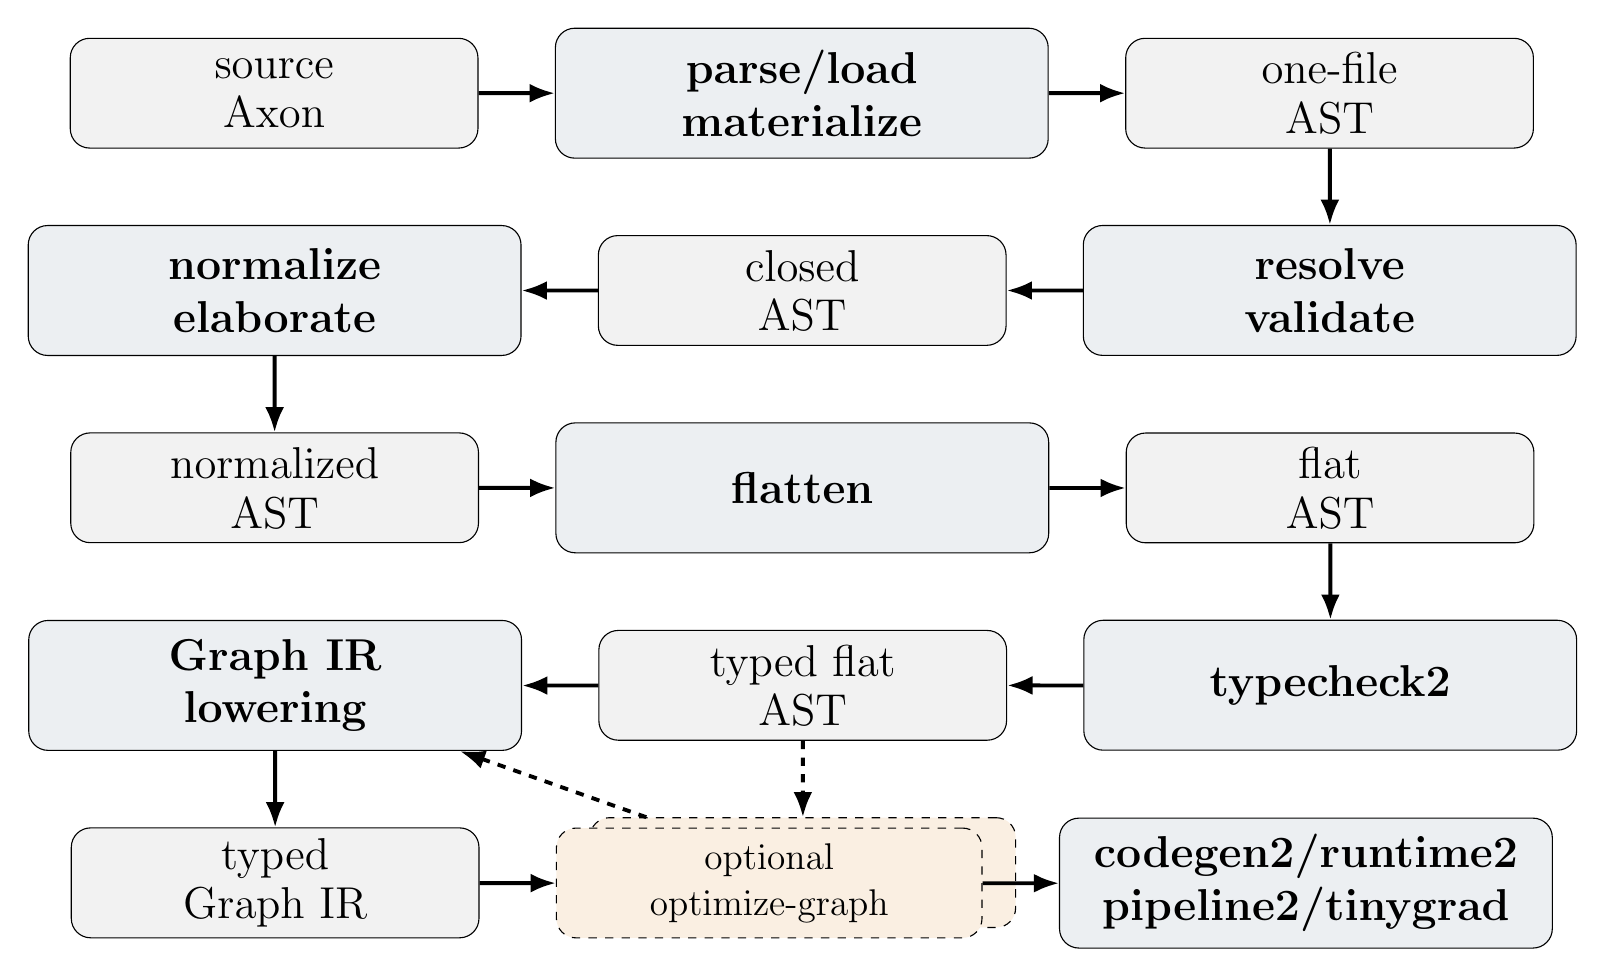
\begin{tikzpicture}[
  transform shape,
  scale=1.12,
  stage/.style={draw, rounded corners=7pt, fill=axonblue!8, align=center, minimum width=2.2in, minimum height=0.58in, font=\bfseries\fontsize{15}{17}\selectfont},
  rep/.style={draw, rounded corners=7pt, fill=black!5, align=center, minimum width=1.82in, minimum height=0.49in, font=\fontsize{14}{16}\selectfont},
  opt/.style={draw, rounded corners=7pt, dashed, fill=axonorange!12, align=center, minimum width=1.9in, minimum height=0.49in, font=\fontsize{13}{15}\selectfont},
  edge/.style={-{Latex[length=3.2mm]}, line width=1.4pt}
]
\node[rep] (src) {source\\Axon};
\node[stage, right=0.34in of src] (parse) {parse/load\\materialize};
\node[rep, right=0.34in of parse] (file) {one-file\\AST};
\node[stage, below=0.34in of file] (resolve) {resolve\\validate};
\node[rep, left=0.34in of resolve] (closed) {closed\\AST};
\node[stage, left=0.34in of closed] (norm) {normalize\\elaborate};
\node[rep, below=0.34in of norm] (normast) {normalized\\AST};
\node[stage, right=0.34in of normast] (flatstage) {flatten};
\node[rep, right=0.34in of flatstage] (flat) {flat\\AST};
\node[stage, below=0.34in of flat] (tc) {typecheck2};
\node[rep, left=0.34in of tc] (typed) {typed flat\\AST};
\node[opt, below=0.34in of typed] (astopt) {optional\\optimize-safe};
\node[stage, left=0.34in of typed] (lower) {Graph IR\\lowering};
\node[rep, below=0.34in of lower] (graph) {typed\\Graph IR};
\node[opt, right=0.34in of graph] (gopt) {optional\\optimize-graph};
\node[stage, right=0.34in of gopt] (backend) {codegen2/runtime2\\pipeline2/tinygrad};
\draw[edge] (src) -- (parse);
\draw[edge] (parse) -- (file);
\draw[edge] (file) -- (resolve);
\draw[edge] (resolve) -- (closed);
\draw[edge] (closed) -- (norm);
\draw[edge] (norm) -- (normast);
\draw[edge] (normast) -- (flatstage);
\draw[edge] (flatstage) -- (flat);
\draw[edge] (flat) -- (tc);
\draw[edge] (tc) -- (typed);
\draw[edge,dashed] (typed) -- (astopt);
\draw[edge,dashed] (astopt) -- (lower);
\draw[edge] (typed) -- (lower);
\draw[edge] (lower) -- (graph);
\draw[edge] (graph) -- (gopt);
\draw[edge] (gopt) -- (backend);
\end{tikzpicture}
\end{minipage}
\hfill
\begin{minipage}[t]{0.41\linewidth}
\centering
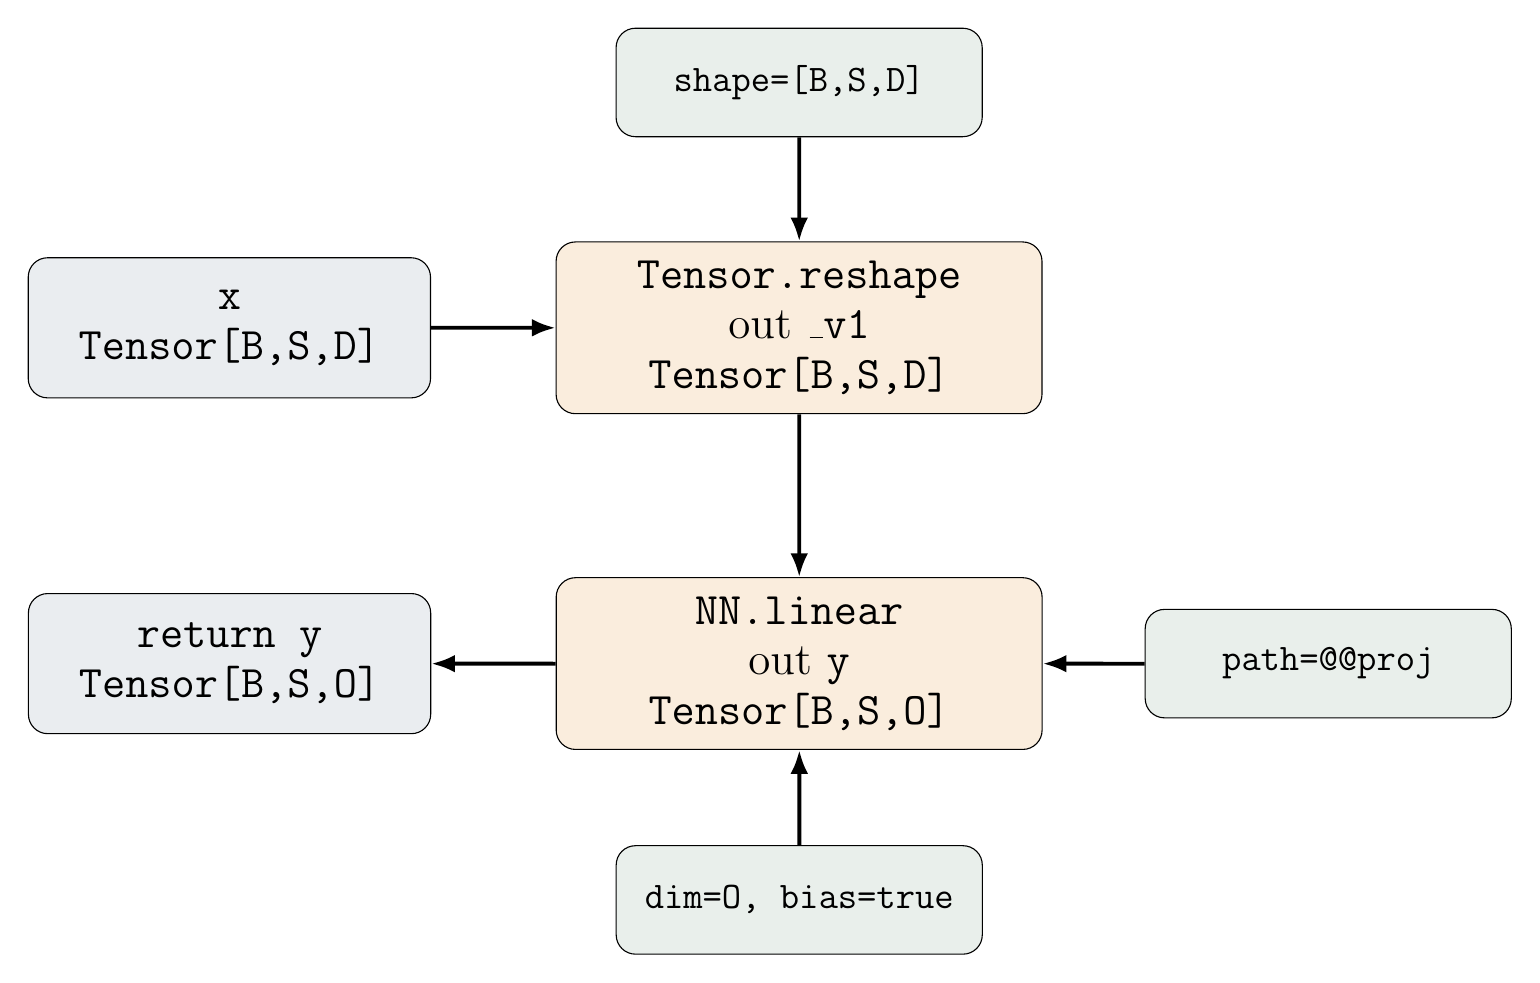
\begin{tikzpicture}[
  transform shape,
  scale=1.13,
  value/.style={draw, rounded corners=7pt, fill=axonblue!9, align=center, minimum width=1.78in, minimum height=0.62in, font=\fontsize{14}{16}\selectfont},
  op/.style={draw, rounded corners=7pt, fill=axonorange!14, align=center, minimum width=2.15in, minimum height=0.76in, font=\fontsize{14}{16}\selectfont},
  attr/.style={draw, rounded corners=7pt, fill=axongreen!12, align=center, minimum width=1.62in, minimum height=0.48in, font=\fontsize{13}{15}\selectfont},
  edge/.style={-{Latex[length=3mm]}, line width=1.4pt}
]
\node[value] (x) {\code{x}\\\code{Tensor[B,S,D]}};
\node[op, right=0.55in of x] (reshape) {\code{Tensor.reshape}\\out \code{\_v1}\\\code{Tensor[B,S,D]}};
\node[op, below=0.72in of reshape] (linear) {\code{NN.linear}\\out \code{y}\\\code{Tensor[B,S,O]}};
\node[value, left=0.55in of linear] (ret) {\code{return y}\\\code{Tensor[B,S,O]}};
\node[attr, above=0.46in of reshape] (shape) {\code{shape=[B,S,D]}};
\node[attr, right=0.45in of linear] (path) {\code{path=@@proj}};
\node[attr, below=0.42in of linear] (attrs) {\code{dim=O, bias=true}};
\draw[edge] (x) -- (reshape);
\draw[edge] (reshape) -- (linear);
\draw[edge] (linear) -- (ret);
\draw[edge] (shape) -- (reshape);
\draw[edge] (path) -- (linear);
\draw[edge] (attrs) -- (linear);
\end{tikzpicture}
\vspace{3mm}

{\raggedright\fontsize{21}{27}\selectfont
\begin{itemize}
\setlength\itemsep{1mm}
\item typed module inputs and named outputs
\item multi-output nodes, e.g. \code{Tensor.chunk}
\item symbolic dims, optional/cache shapes, constraints
\item structured paths and template symbols, not backend strings
\end{itemize}
}
\end{minipage}
\end{tcolorbox}

\vspace{8mm}

\begin{tcolorbox}[posterbox,title={Full GPT-2 KV Axon Model}]
\begin{tcolorbox}[accentbox]
{\raggedright\fontsize{21}{26}\selectfont
\textbf{Complete cached decoder-only model family.}
The source defines token/position embeddings, cached attention, MLP blocks,
layer iteration, and tied output projection. Later stages make scopes, loops,
defaults, paths, and inferred types explicit before lowering to typed \graphir{}.
\hfill\textbf{Path:} \code{gpt2-kv.axon} $\rightarrow$ typecheck2 $\rightarrow$ \graphir{} $\rightarrow$ codegen2/runtime2/pipeline2.\par}
\end{tcolorbox}
\vspace{2mm}
\begin{minipage}[t]{0.49\linewidth}
\vspace{0pt}
\begin{tcolorbox}[codebox]
\begin{lstlisting}[basicstyle=\ttfamily\fontsize{16.8}{18.2}\selectfont]
{-# CHECKPOINTS "openai-community/gpt2" #-}
{-# TASK "causal_lm" #-}

import Activations (gelu_new)
import Attention (attention, merge_heads, reshape_heads)
import Masking (causal_mask)
import Positions (position_ids)
import Cache (Cache, CacheLayer)
import NN
import Tensor

CONTEXT_SIZE = 1024
MODEL_DIM = 768
NUM_LAYERS = 12
NUM_HEADS = 12

gpt2_block :: Tensor[B,S,D] -> ?Tensor[B,K] -> ?CacheLayer[B,H,P,DH] ->
  (Tensor[B,S,D], ?CacheLayer[B,H,K,DH])
gpt2_block x attn_mask past_kv = do
  x1 <- NN.layernorm@ln_1 x
  a, new_kv <- scope@attn do
    q_lin, k_lin, v_lin <-
      NN.linear@c_attn x1 dim=(3 * MODEL_DIM) bias=true transpose=true
      |> Tensor.chunk parts=3
    q <- reshape_heads q_lin heads=NUM_HEADS
    k <- reshape_heads k_lin heads=NUM_HEADS
    v <- reshape_heads v_lin heads=NUM_HEADS
    k, v, new_kv <- Cache.update past_kv k v
    mask <- causal_mask q k window=CONTEXT_SIZE padding_mask=attn_mask
    a <- attention q k v mask
      |> merge_heads
      |> NN.linear@c_proj dim=MODEL_DIM bias=true transpose=true
    return a, new_kv
  x <- x + a
  x3 <- NN.layernorm@ln_2 x
  m <- scope@mlp do
    return NN.linear@c_fc x3 dim=(4 * MODEL_DIM) bias=true transpose=true
      |> gelu_new
      |> NN.linear@c_proj dim=MODEL_DIM bias=true transpose=true
  return x + m, new_kv
\end{lstlisting}
\end{tcolorbox}
\end{minipage}
\hfill
\begin{minipage}[t]{0.49\linewidth}
\vspace{0pt}
\begin{tcolorbox}[codebox]
\begin{lstlisting}[basicstyle=\ttfamily\fontsize{16.8}{18.2}\selectfont]
-- main entry point

gpt2 :: Tensor.TokenIds[B,S] -> ?Tensor[B,K] -> ?Cache[B,H,P,DH] -> ?Bool ->
  (Tensor[B,S,V], ?Cache[B,H,K,DH])
gpt2 input_ids attn_mask past_kv use_cache = do
  tok <- NN.embedding@wte input_ids dim=MODEL_DIM
  pos <- position_ids input_ids attn_mask=attn_mask
           past_length=(Cache.past_length past_kv) pad_fill=1
      |> NN.embedding@wpe
  x <- tok + pos
  new_kv <- use_cache ? Cache.init : null
  x, new_kv <- for@h i <- [0..NUM_LAYERS)
      carry (x, new_kv) do
    past_i <- Cache.index past_kv i
    x, new_i <- gpt2_block x attn_mask past_i
    new_kv <- Cache.append new_kv new_i
    yield x, new_kv
  logits <- NN.layernorm@ln_f x |> NN.linear@wte
  return logits, new_kv
\end{lstlisting}
\end{tcolorbox}
\begin{tcolorbox}[accentbox]
{\raggedright\fontsize{20}{25}\selectfont
\textbf{What later stages add:} lexical scopes become absolute or templated
paths; the loop becomes typed recursion; defaults are explicit; every expression
has a type, arity, and shape annotation; the backend consumes a typed graph, not
rendered strings.\par}
\end{tcolorbox}
\end{minipage}
\end{tcolorbox}

\vspace{8mm}

\begin{tcolorbox}[posterbox,title={Backends and Future Directions}]
{\raggedright\fontsize{22}{28}\selectfont
\begin{minipage}[t]{0.49\linewidth}
\begin{itemize}
\setlength\itemsep{1mm}
\item \textbf{codegen2-torch:} direct PyTorch from typed \graphir.
\item \textbf{runtime2-torch:} interpreter-style debugging from the same graph.
\item \textbf{pipeline2-torch:} graph partitioning and parameter placement.
\item \textbf{codegen2-tinygrad:} separate backend, same graph semantics.
\end{itemize}
\end{minipage}
\hfill
\begin{minipage}[t]{0.49\linewidth}
\begin{itemize}
\setlength\itemsep{1mm}
\item \textbf{Optimization:} safe AST cleanup; broader rewrites on \graphir.
\item \textbf{Distribution:} native processes or DTensor-style layouts.
\item \textbf{Training:} backend-native autograd with graph parameter metadata.
\item \textbf{Dtypes:} bf16/fp16, FP8, MXFP4, NVFP4 capability planning.
\end{itemize}
\end{minipage}
}
\end{tcolorbox}

\vspace{7mm}

\noindent
\begin{minipage}[t]{0.49\linewidth}
\begin{tcolorbox}[posterbox,title={Validation and Roundtrips}]
{\raggedright\fontsize{21}{27}\selectfont
\begin{itemize}
\setlength\itemsep{1mm}
\item Each major stage has a contract: closed names, normalized calls, flat eager control, typed expressions, and graph dependencies.
\item Weak roundtrips check rendering stability at a stage boundary.
\item Strong roundtrips re-run all previous stages from rendered Axon and compare the resulting representation.
\item Fidelity tests compare generated logits against HF references; compiler changes must preserve model-family behavior.
\end{itemize}
}
\end{tcolorbox}
\end{minipage}
\hfill
\begin{minipage}[t]{0.49\linewidth}
\begin{tcolorbox}[posterbox,title={Graph Contract}]
{\raggedright\fontsize{21}{27}\selectfont
\begin{itemize}
\setlength\itemsep{1mm}
\item No Synapse YAML as an IR: lowering emits typed graph modules directly.
\item Structured parameter paths and template symbols remain first-class graph data.
\item Multi-output calls, tuple/list values, optionals, symbolic dims, and constraints are represented semantically.
\item Optimizations should be validated on graph inputs and outputs before code generation.
\end{itemize}
}
\end{tcolorbox}
\end{minipage}

\vfill
\begin{center}
{\fontsize{24}{29}\selectfont\bfseries Compiler invariant: model-family source remains readable; every backend sees the same closed, flat, typed, structured graph.}
\end{center}

\end{document}
